\documentclass[12pt, a4paper, twoside]{report}

% ======================================== Encodage et Langue ========================================
\usepackage[utf8]{inputenc}
\usepackage[T1]{fontenc}
\usepackage[french]{babel}
\usepackage[babel=true]{csquotes}
\frenchsetup{IndentFirst=false}
\usepackage[backend=bibtex, style=numeric]{biblatex}
\addbibresource{biblio.bib}

% ======================================== Typographie et Couleurs ========================================
\usepackage{mathpazo}
\usepackage{helvet}
%\usepackage{fourier}
%\usepackage{libertinus}
\usepackage{xcolor}
\definecolor{mainblue}{RGB}{0, 68, 124}
\definecolor{darkgray}{RGB}{80, 80, 80}

% ======================================== Mise en page ========================================
\usepackage[top=2.5cm, bottom=2.5cm, left=2.5cm, right=2.5cm]{geometry}
\usepackage{graphicx}
\usepackage{setspace}
\setstretch{1.15}
\usepackage[printonlyused, withpage]{acronym}
\usepackage{booktabs}
\usepackage{multirow}
\usepackage{float}
\usepackage{pdfpages}
\usepackage{etoc}
\usepackage{hyperref}
\hypersetup{
    colorlinks=true,       % Remplace les cadres moches par du texte coloré
    linkcolor=mainblue,    % Couleur des liens internes (sommaire, \ref)
    citecolor=mainblue,    % Couleur des citations (\cite)
    urlcolor=mainblue,     % Couleur des liens web (\url)
    pdftitle={Rapport de Stage M1},   % Métadonnée du PDF
    pdfauthor={Mathis Francine-Habas} % Métadonnée du PDF
}

% ================================================================================
% PACKAGES POUR LES MATHS, LE CODE ET L'ALGO
% ================================================================================

% --- Mathématiques ---
\usepackage{amsmath, amssymb, amsthm}
\usepackage[most]{tcolorbox}
\numberwithin{equation}{section}
\usepackage{algorithm}
\usepackage{algpseudocode}

% Définition de couleurs douces pour les fonds
\definecolor{bgcode}{RGB}{248, 248, 248}
\definecolor{bgmath}{RGB}{246, 249, 252}

% Configuration des boîtes mathématiques
\tcbset{
	mathstyle/.style={
		enhanced,
		colback=bgmath,
		colframe=mainblue,
		boxrule=0.8pt,
		arc=3pt,
		left=5pt, right=5pt, top=5pt, bottom=5pt,
		fonttitle=\sffamily\bfseries,
		coltitle=white,
		attach boxed title to top left={yshift=-2mm, xshift=3mm},
		boxed title style={colback=mainblue, arc=2pt, boxrule=0pt}
	}
}

% Création des environnements mathématiques
\newtcbtheorem[number within=section]{theoreme}{Théorème}{mathstyle}{thm}
\newtcbtheorem[number within=section]{definition}{Définition}{mathstyle}{def}
\newtcbtheorem[number within=section]{propriete}{Propriété}{mathstyle}{prop}

\newtcolorbox{preuve}{
	empty,
	borderline west={2pt}{0pt}{mainblue!60},
	left=10pt,
	title={\textit{\textbf{Preuve.}}},
	coltitle=black,
	detach title,
	before upper={\tcbtitle\quad}
}

% --- Code Informatique (C++) ---
\usepackage{listings}
\lstset{
	language=C++,
	backgroundcolor=\color{bgcode},
	basicstyle=\ttfamily\footnotesize,
	keywordstyle=\color{mainblue}\bfseries,
	stringstyle=\color{darkgray},
	commentstyle=\color{teal}\itshape,
	numbers=left,
	numberstyle=\tiny\color{gray},
	stepnumber=1,
	numbersep=8pt,
	frame=l,
	framesep=5pt,
	rulecolor=\color{mainblue},
	breaklines=true,
	tabsize=4,
	showstringspaces=false
}

% --- Pseudo-Code ---
%\usepackage[french, ruled, vlined]{algorithm2e}
%\SetKwInput{KwData}{Données}
%\SetKwInput{KwResult}{Résultat}
%\SetAlFnt{\small}
%\SetAlCapFnt{\small\sffamily}

% --- Design des titres de chapitres ---
\usepackage{titlesec}
\titleformat{\chapter}[display]
{\normalfont\sffamily\Huge\bfseries\color{mainblue}}
{\chaptertitlename\ \thechapter}{10pt}{\Huge}[\vspace{0.5ex}\titlerule]
\titlespacing*{\chapter}{0pt}{-20pt}{30pt}
\titleformat{\section}
{\normalfont\sffamily\Large\bfseries\color{mainblue}}{\thesection}{1em}{}
\titleformat{\subsection}
{\normalfont\sffamily\large\bfseries\color{mainblue}}{\thesubsection}{1em}{}
\titleformat{\subsubsection}
{\normalfont\sffamily\normalsize\bfseries\color{mainblue}}{\thesubsubsection}{1em}{}

% --- En-têtes et Pieds de page ---
\usepackage{fancyhdr}
\pagestyle{fancy}
\fancyhf{}
\renewcommand{\chaptermark}[1]{\markboth{#1}{}}

% Configuration selon ta demande :
% À droite (RO, RE) : Logo + Nom de la fac (sur toutes les pages sauf début de chapitre)
\fancyhead[RO,RE]{
	\begin{tabular}{r}
		\raisebox{-0.3\height}{
\includegraphics[height=1cm]{images/inst5.png}}
	\end{tabular}
}

% À gauche : Alternance (LO = Left Odd / LE = Left Even)
\fancyhead[LO]{\textcolor{mainblue}{\sffamily \textbf{Rapport de Stage}}}
\fancyhead[LE]{\textcolor{mainblue}{\sffamily \textbf{Mathis Francine-Habas}}}

% Pied de page : Numéro au centre
\fancyfoot[C]{\sffamily \thepage}

% Ligne de séparation de l'en-tête
\renewcommand{\headrulewidth}{0.5pt}
\renewcommand{\headrule}{\hbox to\headwidth{\color{mainblue}\leaders\hrule height \headrulewidth\hfill}}

\renewcommand{\thesection}{\Roman{section}}
\renewcommand{\thesubsection}{\thesection.\Roman{subsection}}
\renewcommand{\thesubsubsection}{\thesubsection.\Roman{subsubsection}}
\renewcommand{\theparagraph}{\thesubsubsection.\Roman{paragraph}}

\setcounter{secnumdepth}{3}
\setcounter{tocdepth}{3}

% MATHS SHORTHANDS
\newcommand{\C}{\mathbb{C}}
\newcommand{\R}{\mathbb{R}}
\newcommand{\Q}{\mathbb{Q}}
\newcommand{\Z}{\mathbb{Z}}
\newcommand{\N}{\mathbb{N}}
\newcommand{\U}{\mathbb{U}}
\newcommand{\K}{\mathbb{K}}
\newcommand{\M}{\mathcal{M}}
\newcommand{\B}{\mathcal{B}}
\renewcommand{\epsilon}{\varepsilon}
\renewcommand{\phi}{\varphi}
\renewcommand{\rho}{\varrho}

\newcommand{\mba}{méthode de \textit{BA} }
\newcommand{\mbae}{méthode de \textit{BAE } }
\newcommand{\mmx}{\textbf{MinMax} }
\newcommand{\adv}{\textbf{Adv} }

% --- Paragraphes ---
%\setlength{\parindent}{1.5em} % Tabulation pour les paragraphes suivants
%\setlength{\parskip}{0.4em}   % Espace léger entre les paragraphes

% ======================================== DÉBUT DU DOCUMENT ========================================
\begin{document}
	
	\pagenumbering{roman}
	
	% ======================================== PAGE DE GARDE ========================================
	\begin{titlepage}
		\pagecolor{white}
		
		\noindent
		\begin{minipage}[t]{0.48\textwidth}
			\centering
			
\includegraphics[width=4cm, height=2cm, keepaspectratio]{images/inst5.png} \\
			\vspace{0.2cm}
			\textbf{\small École Nationale de l'Aviation Civile} \\
			\textit{\footnotesize 7 Av. Édouard Belin \\ 31400 Toulouse Cedex 9}
		\end{minipage}
		\hfill
		\begin{minipage}[t]{0.48\textwidth}
			\centering
			
\includegraphics[width=4cm, height=2cm, keepaspectratio]{images/inst1_1.png} \\
			\vspace{0.2cm}
			\textbf{\small Institut de Recherche en Informatique de Toulouse} \\
			\textit{\footnotesize Cr Rose Dieng-Kuntz \\ 31400 Toulouse}
		\end{minipage}
		
		\vspace{1cm}
		
		\noindent
		\begin{minipage}[t]{0.48\textwidth}
			\centering
			
\includegraphics[width=4cm, height=2cm, keepaspectratio]{images/inst3.png} \\
			\vspace{0.2cm}
			\textbf{\small LAAS-CNRS} \\
			\textit{\footnotesize 7 Avenue du Colonel Roche \\ 31400 Toulouse}
		\end{minipage}
		\hfill
		\begin{minipage}[t]{0.48\textwidth}
			\centering
			
\includegraphics[width=4cm, height=2cm, keepaspectratio]{images/inst4.png} \\
			\vspace{0.2cm}
			\textbf{\small Artificial and Natural Intelligence Toulouse Institute} \\
			\textit{\footnotesize 3 Rue Tarfaya \\ 31400 Toulouse}
		\end{minipage}
		
		\vspace{2.5cm}
		
		\begin{center}
			{\color{mainblue}\rule{\textwidth}{2pt}} \\[0.6cm]
			{\sffamily \Huge \bfseries Amélioration de Méthodes de Benders pour un Problème de Planification Robuste sous Incertitude} \\[0.4cm] 
			%{\sffamily \Large Rapport de Stage -- Master 1 IMAI / ROO} \\[0.4cm]
			{\color{mainblue}\rule{\textwidth}{2pt}}
		\end{center}
		
		\vspace{1.5cm}
		
		\begin{center}
			{\Large \textbf{Mathis FRANCINE-HABAS}} \\[1cm]
			
			\begin{tabular}{ll}
				\textbf{Encadrants:} & Christian Artigues \hfill (Directeur de Recherche au LAAS-CNRS) \\
				& Romain Guillaume \hfill (Enseignant-Chercheur à l'IRIT/ANITI) \\[0.3cm]
				\textbf{Tuteur Universitaire:} & Mohammed Sbihi \hfill (Enseignant-Chercheur à l’ENAC)
			\end{tabular}
		\end{center}
		
		\vfill
		
		\begin{center}
			{\large \textbf{Soutenu le :} 27 / 08 / 2026} \\
			\vspace{0.2cm}
			{\large 2025-2026}
		\end{center}
	\end{titlepage}
	
	% ======================================== REMERCIEMENTS ========================================
	\clearpage
	\newgeometry{top=4cm, bottom=4cm, left=3.5cm, right=3.5cm} 
	\thispagestyle{empty}
	
	\vspace*{\fill}
	
	\begin{center}
		{\sffamily \Huge \bfseries \textcolor{mainblue}{Remerciements}} \\[1.5cm]
	\end{center}
	
	\begin{spacing}{2}
		%Je tiens à remercier toutes les personnes qui ont contribué, de près ou de loin, à la réalisation de ce stage et à la rédaction de ce rapport.
		
		%Je remercie tout particulièrement Messieurs Christian Artigues et Romain Guillaume pour la confiance qu'ils m'ont accordée ainsi que pour leur aide tout au long de ce projet de recherche.
		
		%Je souhaite également remercier l'ensemble de mes professeurs pour la qualité de leur enseignement, qui m'ont permis d'acquérir les connaissances nécessaires à la réussite de ma formation et de ce stage.
	\end{spacing}
	
	%\vspace{1.5cm}
	%\begin{flushright}
	%    \textit{Mathis FRANCINE-HABAS}
	%\end{flushright}
	
	\vspace*{\fill}
	
	\clearpage
	\restoregeometry
	
	% ======================================== SOMMAIRES ========================================
	\clearpage
	\tableofcontents
	\thispagestyle{empty}
	
	\clearpage
	% \begin{figure}...\caption{}...\end{figure})
	\listoffigures
	
	\clearpage
	% \begin{table}...\caption{}...\end{table})
	\listoftables
	
%	\clearpage
%	\section*{List of Acronyms}
%	%\addcontentsline{toc}{section}{List of Acronyms}
%	\begin{acronym}[ANITI]
%		\acro{ANITI}{Artificial and Natural Intelligence Toulouse Institute}
%		\acro{LAAS}{Laboratoire d'Analyse et d'Architecture des Systèmes}
%		\acro{PLNE}{Programmation Linéaire en Nombres Entiers}
%		\acro{BA}{Benders Adverse}
%		\acro{BAE}{Benders Adverse Étendu}
%		\acro{OR}{Optimisation Robuste}
%	\end{acronym}
	
	% ======================================== CONTENU DU RAPPORT ========================================
	\clearpage
	\pagenumbering{arabic}
	
	
	% ============================== INTRODUCTION ============================== 
	\section*{Introduction}
	
	Historiquement issue des stratégies militaires de la Seconde Guerre mondiale, la Recherche Opérationnelle (RO) s'est depuis imposée comme la discipline scientifique incontournable pour l'allocation optimale des ressources et l'amélioration des processus industriels.
	Son efficacité actuelle repose sur un triptyque fondamental. Le premier axe consiste à modéliser mathématiquement ces processus complexes afin d'en traduire fidèlement les contraintes et les objectifs.
	Le deuxième réside dans le développement de méthodes de résolution capables de passer à l'échelle industrielle. Enfin, le dernier levier de performance, devenu central aujourd'hui, est le traitement intégré et intelligent des données.
	
	C'est précisément sur ce dernier point que la Recherche Opérationnelle converge vers l'Intelligence Artificielle. Cependant, l'exploitation de ces données issues d'environnements réels confronte systématiquement les modèles à un défi majeur: l'omniprésence de l'incertitude.
	En effet, l'instabilité de la demande, des prix et du climat complexifie la planification au quotidien. La production, la logistique et les approvisionnements subissent des risques accrus, amplifiés par l'interdépendance des chaînes mondiales.
	Les modèles classiques supposent souvent un monde \enquote{parfait}. Optimiser ce scénario crée une stratégie fragile qui ne fonctionnera plus au premier aléa. L'enjeu n'est donc plus seulement d'optimiser un plan idéal, mais également d'anticiper les écarts malgré ces incertitudes : c'est la naissance de l'optimisation robuste (OR).
	
	Ce nouveau concept permet de poser un cadre pour décider dans l'incertitude. Nous pourrions le définir de la façon suivante: l'Optimisation Robuste cherche la meilleure décision qui reste faisable et performante, quels que soient les scénarios à venir.
	Nous avons deux types d'incertitude : elles peuvent être continues ou discrètes. Les incertitudes s'appuient sur des métriques ainsi que sur des scénarios critiques identifiés.
	Les applications couvrent notamment la supply chain, la maintenance et la production, où les aléas locaux peuvent déclencher des effets systémiques sur les performances globales.
	
	Pour résoudre ces problèmes d'Optimisation Robuste, il existe de nombreuses approches. L'une d'entre elles, appelée la méthode de Benders Adverse (BA) (ou parfois méthode des plans coupants) a été introduite dans \cite{Mutapcic01062009}. C'est cette approche que nous avons utilisé et que nous détaillerons par la suite.
	
	Comment les méthodes de Benders peuvent-elles optimiser la planification robuste sous incertitude?
	Nous présenterons tout d'abord le contexte de la recherche, ferons un point sur les avancées scientifiques dans ce domaine, puis nous exposerons les objectifs, les solutions ainsi que les résultats obtenus. Les apports techniques et professionnels de cette expérience feront l’objet de la dernière partie.
	
	
	% ============================== CONTEXTE DE LA RECHERCHE ==============================
	\clearpage
	\section{Contexte de la recherche}
	
	Ce stage s'inscrit au cœur d'un écosystème scientifique toulousain riche, structuré autour d'une collaboration entre trois acteurs majeurs de la recherche en intelligence artificielle et en informatique : l'institut ANITI, l'IRIT-CNRS et le LAAS-CNRS.
	
	L'impulsion de cette dynamique est notamment portée par la chaire HEROIC\footnote{Hybridizing Learning, seaRch and combinatorial Optimization for Industrial deCision-making.} d' ANITI (Artificial and Natural Intelligence Toulouse Institute), un cluster labellisé par la Communauté d'universités et d'établissements de Toulouse. Son ambition est de concevoir des systèmes d'Intelligence Artificielle dont les prises de décision sont explicables, équitables, fiables et robustes, une condition indispensable pour permettre leur déploiement dans des secteurs critiques à haut risque.
	
	Cette volonté de développer des systèmes décisionnels de confiance s'appuie sur l'expertise de deux laboratoires. D'une part, l'Institut de Recherche en Informatique de Toulouse (IRIT), une unité de recherche publique placée sous la tutelle conjointe du Centre National de la Recherche Scientifique (CNRS) et des universités toulousaines. D'autre part, le Laboratoire d'Analyse et d'Architecture des Systèmes (LAAS) est une unité propre du CNRS. Si le LAAS aborde des thématiques très variées, allant de la robotique aux micro-nano-bio-technologies, il se distingue particulièrement par sa recherche théorique et méthodologique sur la conception de lois mathématiques appliquées à la commande et à la décision.
	
	C'est à l'intersection de ces institutions, et plus spécifiquement au sein de l'équipe ROC (Recherche sur des problèmes d'Optimisation Combinatoire) du LAAS, que s'est déroulé mon stage. Positionnée à la frontière entre la Recherche Opérationnelle et l'Intelligence Artificielle, cette équipe offre un cadre scientifique idéal pour aborder les problématiques d'optimisation robuste qui font l'objet de ce rapport.

    Plus précisément, les travaux menés s'inscrivent dans la continuité directe de la thèse de Tom Portoleau (voir \cite{portoleauTHESIS}), soutenue au sein de cette même équipe. L'objectif est d'approfondir et de consolider la méthode de Benders Adverse Étendue qu'il a introduite, en surmontant ses limites combinatoires actuelles. À terme, les modèles d'optimisation et les heuristiques développés ont pour ambition d'être transférés vers l'industrie aéronautique, en partenariat avec Airbus. L'exploitation de ces algorithmes sur des données réelles permettra de tester leur robustesse et leur passage à l'échelle face à des problématiques concrètes et critiques de planification.
	
	% ============================== LITTERATURE ==============================
	\clearpage
	\section{Littérature}
	
	L'optimisation robuste absolue (où approche \mmx) de problèmes de planification est complexe. Pour contourner cette difficulté, les auteurs de \cite{JFBENDERS} ont mis au point la méthode dite de Benders Adverse, qui s'appuie sur une décomposition itérative : elle isole un problème Maître, qui planifie la production, et un problème adverse, qui évalue la robustesse de cette planification en cherchant le pire scénario possible.
	
	Dans la littérature, \cite{PATZOLD202020} présentent une variante de cette méthode où les pires scénarios sont calculés de manière approximative tout en garantissant la convergence de l'algorithme. Plus récemment, les travaux de \cite{portoleauROADEF}, sur lesquels s'appuie l'essentiel de notre étude, proposent la méthode de Benders Adverse Étendue, que nous noterons $BAE$ ou $KC$ pour \textit{Knowledge Compilation}. Contrairement à l'approche classique, l'adversaire ne renvoie plus un unique pire cas, mais un ensemble de scénarios défavorables afin d'accélérer la convergence globale. 

    Afin de justifier l'efficacité de cette approche étendue, il est nécessaire de s'appuyer sur le paradigme de la Compilation de Connaissances (KC). Initialement issue de l'intelligence artificielle et de l'informatique théorique \cite{Darwiche_2002}, la KC consiste à compiler une théorie propositionnelle complexe (ici, l'espace des scénarios incertains) dans un langage cible qui est structuré, typiquement un Graphe Orienté Acyclique (DAG). 
    
    Comme démontré par Darwiche et Marquis \cite{Darwiche_2002}, l'intérêt majeur des DAGs réside dans leur capacité à trouver un compromis idéal entre la précision et la tractabilité. En imposant des propriétés structurelles telles que la \textit{décomposabilité} (où les sous-problèmes traitent de variables disjointes), le DAG permet de factoriser les redondances qui sont présentes dans une formulation de type CNF (\textit{Conjunctive Normal Form}). Cette factorisation rend possible l'utilisation d'algorithmes permettant l'agrégation de scénarios en temps polynomial. %rajoter: par rapport à la taille du graphe, et non par rapport à l'exponentielle de l'espace de décision.
    
    Dans le domaine de l'Optimisation Combinatoire (OC), cette logique a été transposée aux Diagrammes de Décision (\textit{Decision Diagrams for Optimization}) \cite{bergman2016decision}. Dans la méthode de Benders classique, l'énumération itérative de scénarios discrets se traduit par l'ajout de contraintes linéaires indépendantes, potentiellement redondantes, qui saturent rapidement le problème Maître. À l'inverse, l'approche KC proposée par \cite{portoleauTHESIS} exploite la décomposabilité du DAG pour agréger ces scénarios défavorables. Au lieu de stocker chaque scénario individuellement, la méthode factorise leurs sous-chemins communs au sein d'une structure unique (que nous définirons par la suite comme le graphe partiel de budget). Cette factorisation réduit le nombre de variables et de contraintes générées à chaque itération, permettant ainsi de limiter le phénomène d’explosion combinatoire tout en conservant l'information nécessaire et suffisante.
    
    Dans la continuité de cette recherche, nous présenterons cette méthode pour un problème de dimensionnement de lots avec contraintes de capacité (\textit{Capacitated Lot Sizing- Problem - CLSP}), soumis à un budget d'incertitude portant sur la demande cumulée.

    \subsection{Définition et Modélisation du Problème}
	
	Afin de modéliser ce problème, nous considérons un horizon de planification divisé en $T$ périodes. A chaque période $t\leq T$, la demande est notée $d_t$ et la quantité produite $x_t$. Un plan de production est constitué par l'ensemble de ces variables décisionnelles sur l'horizon. La production, à chaque pas de temps, est bornée par une capacité maximale $\mathbb{X}$, de sorte que $x_t\leq \mathbb{X}$. La gestion des flux de production génère différents coûts linéaires indépendants de la période. On a $c^P$ le coût unitaire de lancement de production, $c^I$ le coût unitaire de stockage appliqué au surplus de production (noté $I_t$), $c^B$ le coût unitaire de pénalité de retard appliqué à la demande insatisfaite (notée $B_t$), et enfin $b^P$ le prix de vente unitaire appliqué à la quantité de demande effectivement satisfaite (notée $s_t$). Contrairement aux approches classiques où l'incertitude porte sur la demande de chaque période de façon indépendante, notre modèle intègre une incertitude sur la demande \textbf{cumulée}. Soient $X_t = \sum_{i=1}^{t}x_i$ la production cumulée et $D_t = \sum_{i=1}^{t}d_i$ la demande cumulée à l'instant $t$. L'incertitude sur la demande cumulée est modélisée par un intervalle symétrique  $[\hat{\mathcal{D}}_t - \Delta_t, \hat{\mathcal{D}}_t + \Delta_t]$, où $\hat{\mathcal{D}}_t \geq \Delta_t \geq 0$ représente la valeur nominale et $\Delta_t$ la déviation maximale.
	
	Nous définissons un \textbf{scénario} comme une réalisation spécifique de ces incertitudes au sein d'un ensemble de scénarios possibles $\mathcal{U}$. En imposant une limite globale sur les déviations via un budget d'incertitude $\Gamma$, l'ensemble continu des scénarios admissibles se définit par :
	
	\begin{equation}
		\mathcal{U} = \left\{ (D_t)_{t\leq T} \mid D_t \leq D_{t+1},\, D_t \in [\hat{\mathcal{D}}_t - \Delta_t, \hat{\mathcal{D}}_t + \Delta_t],\, \vert{}\vert{}\mathcal{D}-\hat{\mathcal{D}}\vert{}\vert{}_1 \leq \Gamma \right\}
	\end{equation}
	
	Ce problème de \textit{lot-sizing} déterministe sous-jacent étant \textit{NP-Difficile} \cite{computational_complexity_gabriel}, sa résolution sous incertitude requiert une approche \mmx.
	
	\subsection{Méthode de Benders Adverse (BA)}
	
	Le principe fondamental de la méthode de Benders Adverse est de résoudre le problème \mmx itérativement. Plutôt que de confronter le modèle à l'infinité des scénarios de $\mathcal{U}$ simultanément, le problème Maître est initialement résolu face à un scénario unique, correspondant à la demande nominale notée $\hat{\mathcal{D}}$.
	
	Une fois le plan de production initial $S$ obtenu, une phase adverse (le sous-problème \adv) est exécutée. Son rôle est d'identifier, pour ce plan $S$ figé, le scénario $\mathcal{D}'$ maximisant les coûts. Ce pire scénario est alors ajouté à l'ensemble restreint des scénarios considérés, et le problème Maître est résolu à nouveau. Ce processus itératif, illustré par la figure \ref{fig:sch_ba}, s'arrête si le critère d'arrêt est atteint, c'est-à-dire lorsque l'adversaire n'est plus en mesure de trouver un scénario dégradant la valeur objective du problème Maître. Le Maître et l'adversaire ont convergé vers la même solution ; cette dernière est donc robuste.
	
	\begin{Figure}[H]
		\centering
		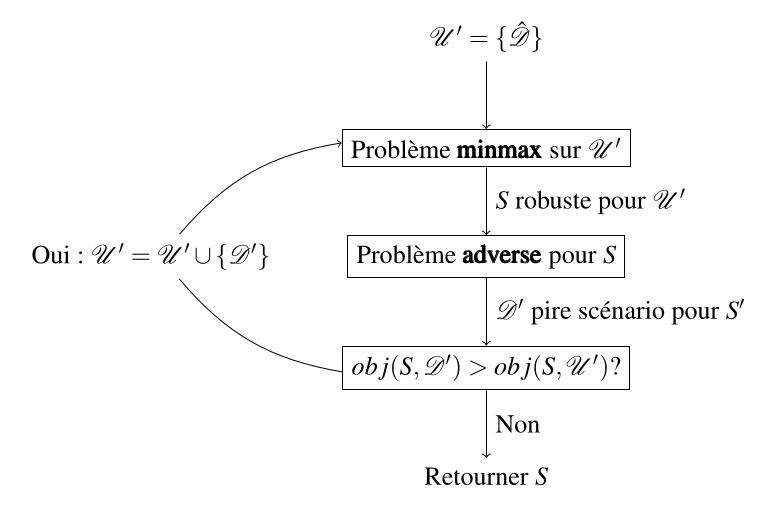
\includegraphics[width=0.7\linewidth]{images/schema_ba.png} 
		\caption{Schéma de la méthode de Benders Adverse. \cite{portoleauROADEF}}
		\label{fig:sch_ba}
	\end{figure}
	
	Pour appliquer cette méthode à notre problème, il faut donc être capable de résoudre le problème \mmx pour une liste de scénarios donnée et de résoudre le problème \adv pour une solution du problème donné.
	
	\subsubsection{Le problème \mmx}
	
	L'objectif du problème Maître est de trouver le plan de production minimisant les coûts face au pire des scénarios connus. Mathématiquement, il s'agit de résoudre \\ $\min_{X \in \mathcal{X}} \max_{u \in U} \text{Coût}(X, u)$, où $U \subseteq \mathcal{U}$ est la liste finie des scénarios générés par l'adversaire.
	
	Afin de le modéliser sous la forme d'un \textit{Programme Linéaire en Nombres Entiers Mixtes (MILP)}, une technique de reformulation en épigraphe est employée. On introduit une variable auxiliaire continue $z$ dont le rôle est de majorer le coût total pour l'ensemble des scénarios $l\in U$. En minimisant ce majorant $z$, on minimise le coût du scénario le plus défavorable. Outre $z$, le modèle utilise une variable binaire $y_t\in \{0, 1\}$ indiquant si une production a lieu à la période $t$, et la constante $M$ du \textit{Big-M} pour lier les variables continues et binaires.
	
	\begin{align}
		\label{lot-sizing-prb}
		\min\quad & z \\
		\text{s.t.}\quad & \sum_{t=1}^{T}\left(c^I I_{t,l} + c^B B_{t,l} + c^P y_t - b^P s_{t,l}\right) \le z && l\le |U|,\\
		& B_{t,l}-I_{t,l}=D_t^l-X_t && \forall t\in[T],\ l\le |U|,\\
		& \sum_{i=1}^{t}s_{i,l}=D_t^l-B_{t,l} && \forall t\in[T],\ l\le |U|,\\
		& X_t-X_{t-1}\le My_t && 2\le t\le T,\\
		& X_1\le My_1,\\
		& B_{t,l},\,I_{t,l},\,s_{t,l}\ge0 && \forall t\in[T],\\
		& y_t\in\{0,1\} && \forall t\in[T],\\
		& X\in\mathbb{X}\subseteq\mathbb{R}_+^T
	\end{align}
	
	\vspace{-0.5em}
	{\centering
		\small Lot-Sizing Problem. \cite{portoleauTHESIS}\par
		\label{formulation_probleme_maitre}
	}
	
	Dans notre formulation, la contrainte limitant $z$ garantit le robustesse du modèle. Les contraintes d'équilibres assurent la conservation des flux entre la production cumulée $X_t$ et la demande $D_t^l$, tandis que la somme des ventes $s_{i, l}$ modélise la quantité effectivement écoulée.
	
	\subsubsection{Le sous-problème \adv}
	
	Une fois le plan de production $X$ fixé, le sous-problème cherche a construire le pire scénario entier. Bien que ce problème de maximisation soit \textit{NP-Difficile} au sens faible, \cite{guillaume2020robustproductionplanningbudgeted} ont démontré qu'il pouvait être résolu en temps pseudo-polynomial. L'astuce consiste à modéliser l'espace des déviations de la demande sous la forme d'un graphe acyclique orienté, au sein duquel la recherche du pire scénario se réduit à la recherche du plus long chemin.
	
	\begin{definition}{Graphe de budget}{graphe_budget}
		On note ce graphe $\mathcal{G}=(V, A)$. L'ensemble des noeuds $V$ partitionné en $T+2$ niveaux et, mis à part le premier et le dernier niveau qui contiennent un unique noeud chacun, chaque niveau contient $\Gamma +1$ noeuds. On note respectivement $v_0$ et $v_{T+1}$ les noeuds du premier et du dernier niveau, et $v_{t, i}$ pour $1\leq t\leq T$ et $0\leq i \leq \Gamma$ tous les autres noeuds du graphe. L'ensemble des arcs $A$ est construit de sorte que l'arc de $v_{t-1, i}$ vers $v_{t, j}$ existe et si et seulement si $i\leq j$ et $j-i\leq\Delta_t$ pour chaque $t$ compris entre $1$ et $T$, et un arc de $v_0$ vers $v_{T+1}$ représente un scénario de $\mathcal{U}$, et que si un noeud $v_{t, i}$ est sur ce chemin, alors $i$ unités de budget ont été consommées entre la première période et la période $t$. Ensuite, on définit les coûts des arcs de sorte qu'ils représentent chacun la contribution à la fonction objective de la décision de faire varier la demande à une période donnée pour une solution $X$ donnée. Plus formellement, on définit les coûts des arcs par :
		
		\[
		c_{t-1, i, t, j}=\left\{
		\begin{array}{ll}
			\max\{c^I(X_t-(\hat{\mathcal{D}}_t-(j-i))),\\
			c^B(\hat{\mathcal{D}}_t+(j-i)-X_t)\} + c^Py_t & \text{si}\, 1\leq t\leq T-1,\\
			\max\{c^I(X_t-(\hat{\mathcal{D}}_t-(j-i))) - b^P(\hat{\mathcal{D}}_t - (j-i), \\
			c^B(\hat{\mathcal{D}}_t+(j-i)-X_t) - b^PX_t\} + c^Py_t & \text{si}\, t=T,\\
			0 & \text{si}\, t=T+1
		\end{array}
		\right.
		\]
		
		où $c_{t-1, i, t, j}$ est le coût de l'arc entre les noeuds $v_{t-1, i}$ et $v_{t, j}$ lorsque cet arc existe, et $y_t=0$ si $X_{t-1}=X_t$ et $1$ sinon.
	\end{definition}
	
	De ce fait, évaluer un scénario revient à sommer les poids des arcs traversés, et identifier le pire scénario revient à extraire le chemin de poids maximal dans $\mathcal{G}$ (schématisé en figure \ref{fig:sch_graphe_budget}). Pour la suite du rapport, le terme de \enquote{chemin} signifiera une suite d'arcs dans le graphe entre la source $v_0$ et le puits $v_{T+1}$.
	
	\begin{figure}[H]
		\centering
		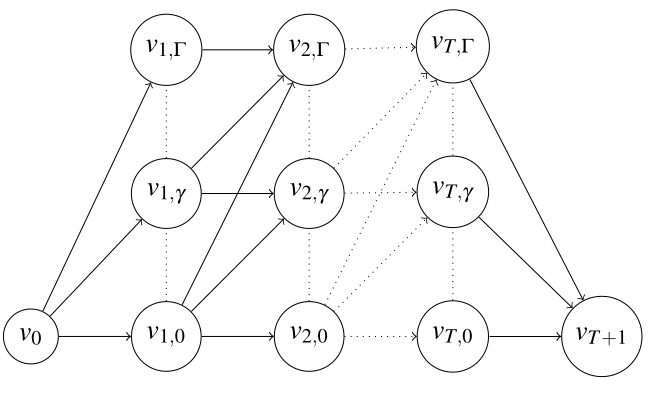
\includegraphics[width=0.7\linewidth]{images/graphe_budget.png} 
		\caption{Schéma générique du graphe de budget. \cite{guillaume2020robustproductionplanningbudgeted}}
		\label{fig:sch_graphe_budget}
	\end{figure}
	
	\subsubsection{L'algorithme de Benders Adverse pour le lot-sizing sous incertitude}
	
	Voici l'algorithme implémenté par \cite{portoleauTHESIS} pour résoudre le problème de Benders Adverse présenté ci-dessus dans la figure \ref{fig:sch_ba}. Tant que l'adversaire parvient à construire un graphe de budget dont le plus long chemin révèle un coût $v'$ strictement supérieur au coût $v$ anticipé par le Maître, ce nouveau scénario est ajouté à $\mathcal{U}$ et le processus réitère.
	
	\begin{algorithm}[H]
		\caption{Adversarial Benders Method}
		\label{alg:benders_algo}
		\begin{algorithmic}[1]
			\State $\mathcal{U} \gets \{\hat{\mathcal{D}}\}$
			\State $(X,v) \gets \Call{SolveMaster}{\mathcal{U}}$
			\State $(\mathcal{D},v') \gets \Call{SolveAdversarial}{X}$
			
			\While{$v \neq v'$}
			\State $v \gets v'$
			\State $\mathcal{U} \gets \mathcal{U} \cup \{\mathcal{D}\}$
			\State $(X,v) \gets \Call{SolveMaster}{U}$
			\State $(\mathcal{D},v') \gets \Call{SolveAdversarial}{X}$
			\EndWhile
			
			\State \Return $(X,v)$
		\end{algorithmic}
	\end{algorithm}
	
	\subsection{Méthode de Benders Adverse Étendu (BAE)}
	
	Cette section détaille la méthode de Benders Adverse Étendue (BAE), formellement introduite par \cite{portoleauTHESIS}. Cette approche constitue le fondement de mes recherches. Il s'agit d'une extension de la méthode de Benders Adverse classique présentée précédemment, conçue pour accélérer la convergence de l'algorithme. Plutôt que d'isoler l'unique pire scénario à chaque itération du sous-problème adverse, la BAE génère un ensemble de scénarios défavorables. L'enjeu de cette méthode réside dans la résolution du problème Maître : sa formulation initiale, basée sur une liste explicite de scénarios  $\mathcal{U}$, souffre d'une explosion combinatoire et passe très difficilement à l'échelle lorsque ce nombre augmente. Pour faire face à cette limite, le problème Maître est redéfini en s'appuyant sur une structure plus compacte : le graphe partiel de budget.
	
	\subsubsection{Le problème \mmx}
	
	Pour ce faire, les auteurs de \cite{portoleauTHESIS} ont précisément défini cette notion. Lorsque le problème Maître du Benders Adverse classique se basait sur l'approximation de l'ensemble des scénarios $\mathcal{U}$ par une liste de scénarios, cette fois-ci, elle se fait par l'extraction d'un sous-graphe issu du graphe de budget global (voir \ref{fig:sch_graphe_budget}).
	
	\begin{definition}{Graphe partiel de budget}{graphe_partiel_budget}
		Soit $\mathcal{G}=(V, A)$ un graphe de budget défini suivant la Définition~\ref{def:graphe_budget}. On dit que $\mathcal{G}'=(V, A')$ est un graphe partiel de budget de $\mathcal{G}$ si $A'\subset A$ et pour tout arc $a\in A'$, il existe un chemin de $v_0$ vers $v_{T+1}$ passant par l'arc $a$. Les poids des arcs de ce graphe sont calculés de la même manière que pour le graphe défini précédemment. On a alors $\mathcal{U}_{\mathcal{G}'}\subset \mathcal{U}_{\mathcal{G}}$.
	\end{definition}
	
	Grâce à cette structure, le problème Maître peut être reformulé comme un problème de calcul de plus long chemin dans le graphe partiel $\mathcal{G}'$. Cette formulation s'appuie sur des variables duales, notées $\pi_{t,i}$, qui représentent le coût du plus long chemin depuis le nœud source $v_0$ jusqu'au nœud $v_{t,i}$. Le programme linéaire en variables mixtes modélisant ce nouveau problème Maître s'écrit alors de la manière suivante :
	
	\begin{align}
		\min\quad & \pi_{T+1}\\
		\text{s.t.}\quad &\pi_{t_j}-\pi_{(t-1)_i} \geq c^I\left(X_t-(\hat{\mathcal{D}}_t-(j-i))\right)+c^P y_t, &&t\in[1,T-1],\ a_{t,i,j}\in A',\\
		&\pi_{t,j}-\pi_{(t-1)_i} \ge c^B\left(\hat{\mathcal{D}}_t+(j-i)-X_t\right)+c^P y_t, &&t\in[1,T-1],\ a_{t,i,j}\in A',\\
		&\pi_{t,j}-\pi_{(t-1)_i} \ge c^I\left(X_t-(\hat{\mathcal{D}}_t-(j-i))\right) +c^P y_t -b^P(\hat{\mathcal{D}}_t-(j-i)), &&t=T,\ a_{t,i,j}\in A',\\
		&\pi_{t_j}-\pi_{(t-1)_i} \geq c^B(\hat{\mathcal{D}}_t + (j-i)-X_t)+c^Py_t-b^PX_t && t=T,\ a_{t,i,j}\in A',\\
		& \pi_{T+1}-\pi_{T, i}\geq 0 && 0\leq i\leq \Gamma,\\
		&\pi_0=0,\, \pi_v\in\mathbb{R} && v\in V,\\
		&X_t-X_{t-1}\leq My_t && 2\leq t \leq T,\\
		& X_1 \leq My_1\\
		& y_t \in \{0, 1\} && 1\leq t\leq T,\\
		& X\in\mathbb{X}
	\end{align}
	
	\vspace{-0.5em}
	{   \centering
		\small Reformulation du problème Maître. \cite{portoleauTHESIS}\par
		\label{reformulation_pbr_maitre}
	}
	
	\subsubsection{Le sous-problème \adv}
	
	Une fois le problème Maître résolu pour une itération donnée, il fournit un plan de production $X$. L'objectif du sous-problème adverse est alors d'évaluer la robustesse de cette solution en cherchant non pas un unique pire scénario, mais un ensemble de scénarios défavorables qui viendront augmenter les connaissances du problème Maître à l'itération suivante. Cet ensemble prend la forme d'un nouveau graphe partiel de budget, noté $\mathcal{G}''$.

	Pour construire ce graphe, la méthode s'appuie sur un algorithme de programmation dynamique (voir \ref{alg:adv_subgraph}). Dans un premier temps, un calcul de plus long chemin est réalisé sur le graphe de budget complet $\mathcal{G}$, afin de déterminer le coût maximal pour atteindre chaque noeud depuis l'origine $v_0$. Cette étape s'effectue rapidement du fait que le graphe soit orienté et sans cycle. Ensuite, une phase de remontée (\textit{backtracking}) est réalisée depuis le noeud final $v_{T+1}$. A chaque étape de cette remontée, au lieu de ne conserver que l'arc menant au pire chemin absolu, l'algorithme sélectionne un sous-ensemble d'arcs appartenant aux chemins critiques. C'est cette sélection d'arcs qui définit la structure et la taille du graphe partiel $\mathcal{G}''$. Pour être plus précis, une heuristique a été mise en place sur la définition des pires chemins. Lors de la première phase, le coût du plus long chemin, noté $C$, va servir de référence pour définir la notion de chemin critique. Considérons $\tau\in[0, 1]$, un chemin critique sera donc un scénario dont sa longueur est supérieure ou égale à $\tau C$ dans le graphe de budget. Si $\tau=1$ alors seuls les chemins ayant le même coût que celui du pire chemin sont considérés comme critiques et donc ajoutés au sous-graphe. A l'inverse, si $\tau=0$, tous les chemins sont considérés comme étant des chemins critiques. Nous nous attendons à ce que la diminution de $\tau$ entraîne une augmentation du temps de résolution mais une potentielle baisse du nombre d'itération.
	
	\begin{algorithm}[H]
		\caption{Adv\_subGraph}
		\label{alg:adv_subgraph}
		\begin{algorithmic}[1]
			\Require $\mathcal{G}=(V, A)\, \text{and}\, \tau\in[0, 1]$
			\Ensure $\mathcal{G}'=(V, A), \pi_{T+1}$
			
			\State $\pi_0 \gets 0$
			\For{$t=1 \rightarrow T+1$}
			\For{$j=0 \rightarrow \Gamma+1$}
			\State $\pi_{t, j} \gets \max\{\pi_{t-1, i}+c_{t-1, i, t, j} | (v_{t-1, i}, v_{t, j})\in A\}$
			\EndFor
			\EndFor
			\State $A'=\{\}$
			\For{$t=T \rightarrow 1$}
			\For{$j=0 \rightarrow \Gamma+1$}
			\If{$\pi_{T, j}\geq \tau\pi_{T+1}\text{and}t=T$}
			\State $A'\gets A'\cup \{(v_{T, j}, v_{T+1})\}$
			\State $v_{T, j}\gets\text{marqued}$
			\EndIf
			\If{$v_{t, j}\, \text{is marqued}$}
			\For{$i=0 \rightarrow \Gamma+1$}
			\If{$\pi_{t-1, i}+c_{t-1, i, t, j}=\pi_{t, j}$}
			\State $A'\gets A'\cup \{(v_{t-1, i}, v_{t, j}\}$
			\State $v_{t-1, i}\gets \text{marqued}$
			\EndIf
			\EndFor
			\EndIf
			\EndFor
			\EndFor
			
			\State \Return $\mathcal{G}'=(V, A'), \pi_{T+1}$
		\end{algorithmic}
	\end{algorithm}
	
	\subsubsection{L'opération de fusion}
	
	Dans l'approche de Benders Adverse classique, l'ajout d'un nouveau scénario se traduit par une simple concaténation dans une liste. Dans le cadre de la BAE, il est nécessaire de combiner le graphe partiel de l'itération courante ($\mathcal{G}'$) avec celui généré par le sous-problème adverse ($\mathcal{G}''$). La nouvelle opération de fusion a été défini de la manière suivante : $\text{Merge}(\mathcal{G}', \mathcal{G}'')=(V, A'\cup A'')$.
	
	Toutefois, cette opération de fusion soulève une limite, sur laquelle j'ai travaillé, concernant l'aspect combinatoire de cette méthode \cite{portoleauTHESIS} : la fusion de deux graphes partiels peut générer de nouveaux chemins qui n'existaient dans aucun des deux graphes initiaux. Ainsi, l'ensemble des scénarios du graphe fusionné est potentiellement plus grand que la somme des scénarios des graphes de départ. Il devient donc nécessaire de travailler sur l'affinage des coupes combinatoires afin de ne pas perdre l'avantage porté par cette extension.
	
	\subsubsection{Stratégies de sélection des pires scénarios}
	
	Comme évoqué précédemment, la taille et la densité du graphe partiel de budget $\mathcal{G}''$ dépendent entièrement de la politique de sélection des arcs lors de la phase de backtracking. Dans la littérature, deux heuristiques principales ont été proposées pour effectuer ce tri parmi les chemins critiques \cite{portoleauTHESIS} :
	
	\begin{itemize}
		\item $SelectAll$ : Cette approche exhaustive consiste à sélectionner tous les arcs entrants dont les noeuds d'origine appartiennent à l'un des plus longs chemins dans le graphe partiel. Autrement dit, le graphe généré contient l'intégralité des pires scénarios entiers pour la solution courante. Bien qu'elle fournisse une information très complète au problème Maître, cette méthode tend à faire exploser très rapidement le nombre d'arcs après quelques opérations de fusion. Le graphe partiel devient alors trop dense et difficile à exploiter.
		\item $SelectFew$ : Pour faire face à ce problème, cette méthode propose de restreindre la sélection. Lors du parcours, un premier arc critique est systématiquement choisi, puis un autre arc critique potentiel n'est ajouté qu'avec une certaine probabilité, suivant une loi de Bernoulli de paramètre $p$ (les travaux de référence utilisent généralement $p=\frac{1}{T}$, où $T$ est le nombre de périodes dans l'horizon RAJOUTER SOURCE). Cette restriction probabiliste permet de garder un graphe partiel de taille réduite, car il existe un grand nombre de pires scénarios équivalents.
	\end{itemize}
	
	Ces deux méthodes illustrent le compromis soutenu par les auteurs $BAE$. Il s'agit de fournir suffisamment de scénarios critiques au Maître pour le guider efficacement, tout en contrôlant la taille du graphe pour garantir des temps de résolution acceptables. Cette nécessité de filtrage met en évidence l'intérêt de développer des heuristiques de sélection plus structurelles. Au lieu de s'en remettre à une sélection probabiliste ou exhaustive, il devient pertinent de chercher à extraire des chemins non seulement critiques, mais les plus diversifiés possibles, afin de maximiser la quantité d'information transmise tout en minimisant la redondance des scénarios. C'est ce point que nous aborderons dans la prochaine section. Dans la suite du rapport, $BAE$ signifiera l'approche Benders Adverse Étendue avec l'heuristique $SelectAll$, et $BAE_{Few}$ permettra de spécifier l'utilisation de l'heuristique $SelectFew$.
	
	\subsubsection{L’algorithme de Benders Adverse Étendue pour le lot-sizing sous incertitude }
	
	En combinant les éléments précédents, nous avons le schéma itératif de la méthode de Benders Adverse Étendue. De la même manière que nous initialisons l'algorithme de Benders Adverse (voir Algorithme \ref{alg:benders_algo}) par le scénario nominal, ici, nous initialisons la méthode de Benders Adverse Étendue par le graphe de budget $\hat{\mathcal{G}}$ ne contenant que le scénario nominal.
	
	\begin{algorithm}[H]
		\caption{Extended Adversarial Benders Method}
		\label{alg:benders_algo_etendue}
		\begin{algorithmic}[1]
			\State $\mathcal{G}' \gets \hat{\mathcal{G}}$
			\State $(X,v) \gets \Call{SolveMaster}{\mathcal{U}}$
			\State $(\mathcal{G}'',v') \gets \Call{SolveAdversarial}{X}$
			
			\While{$v \neq v'$}
			\State $v \gets v'$
			\State $\mathcal{G}' \gets Merge(\mathcal{G}', \mathcal{G}'')$
			\State $(X,v) \gets \Call{SolveMaster}{\mathcal{U}}$
			\State $(\mathcal{G}'',v') \gets \Call{SolveAdversarial}{X}$
			\EndWhile
			
			\State \Return $(X,v)$
		\end{algorithmic}
	\end{algorithm}
	
	% ============================== TRAVAIL EFFECTUE ==============================
	\clearpage
	\section{Présentation du travail effectué}
	
	% ============================== OBJECTIFS ==============================
	\subsection{Objectifs}
	
	Cette section détaille les objectifs scientifiques de cette recherche, les propositions algorithmiques formulées, ainsi que les résultats expérimentaux obtenus. La démarche globale s'est structurée en trois temps fondamentaux.
	
	\subsubsection{Manipulation théoriques et restructuration du modèle informatique}
	
	La première phase du stage a été consacrée à l'assimilation des concepts d'optimisation robuste appliqués à la problématique du \textit{lot-sizing} sous incertitude. Afin de conceptualiser le fonctionnement de la méthode de Benders Adverse, l'algorithme a d'abord été déroulé et appliqué sur des instances de taille réduite (le détail de ces itérations est consultable en Annexe X).
	
	Au-delà de l'appropriation théorique, une partie de ce travail a reposé sur de l'implémentation logicielle. En effet, après avoir récupéré une version du code en \textit{C++} utilisé dans la thèse de \cite{portoleauTHESIS}, il a été nécessaire de le reconstruire de manière stable. Ce travail de refonte a exigé de modéliser et d'implémenter plusieurs contraintes mathématiques manquantes par rapport à la formulation du problème de \textit{lot-sizing} sus-cité (voir \ref{lot-sizing-prb}), mais également de parfaire la liaison avec le solveur exact \textit{CPLEX} pour garantir la viabilité des expérimentations futures.
	
	
	\subsubsection{Analyse des performances de référence}
	
	Une fois l'environnement de développement opérationnel, l'objectif suivant a été de reproduire les expérimentations de référence pour évaluer le comportement des différentes approches existantes. L'idée défendue par la méthode $BAE$ est que l'extraction d'un graphe de pires scénarios permet de réduire le nombre d'itération afin de gagner en temps de calcul. Pour valider cette première hypothèse, nous avons mené une batterie de tests sur des instances générées aléatoirement via un script créé pour notre problème. Ces instances simulent une planification sur $52$ périodes (représentant une année de production), pour $20$ références de produits distincts. Une périodicité trimestrielle de $13$ semaines a été mise en place. La probabilité qu'une demande à un instant $t$ pour une référence donnée, durant une période dense, suit une loi de Bernoulli de paramètre $p_{demand}=0.5$. La probabilité pour une période creuse est égale à $(1-p)$. L'étude a été réalisée en faisant varier le budget d'incertitude $\Gamma$ dans son ensemble de définition $\mathcal{D}_{\Gamma}=\{1, 11, \cdots, 91, 101\}$, et $\tau=1$. En ce qui concerne l'heuristique de sélection partielle $BAE_{few}$, la décision de conserver un arc alternatif lors du \textit{backtracking} suit également une loi de Bernoulli de paramètre $p_{few}=0.35$ \footnote{Ce paramètre n'a pas fait l'objet d'une étude spécifique.}. Le tableau \ref{tb:res_initiaux} synthétise ces résultats de référence, en mesurant le nombre moyen d'itérations et le temps de résolution en secondes pour les couples de la forme $(\Gamma_i, \{BA\})$ et $(\Gamma_i, \tau, \{BAE_{all}, BAE_{few}\}), \forall i\in\mathcal{D}_{\gamma}$.
	
	\begin{table}[H]
		\label{tb:res_initiaux}
		\centering
		\begin{tabular}{@{}|l|llllll@{}}
			\toprule
			\multirow{2}{*}{$\Gamma$ \textbackslash{} Methode} & \multicolumn{2}{l|}{BA}                                & \multicolumn{2}{l|}{$BAE_{all}$}                              & \multicolumn{2}{l|}{$BAE_{few}$}                              \\ \cmidrule(l){2-7} 
			& iter.                     & time                       & iter.                     & time                       & iter.                     & time                       \\ \midrule
			1                                             & \multicolumn{1}{l|}{3.0} & \multicolumn{1}{l|}{0.224}  & \multicolumn{1}{l|}{\textbf{1.0}} & \multicolumn{1}{l|}{0.007}  & \multicolumn{1}{l|}{\textbf{1.0}} & \multicolumn{1}{l|}{\textbf{0.005}}  \\ \midrule
			21                                            & \multicolumn{1}{l|}{10.0} & \multicolumn{1}{l|}{0.274} & \multicolumn{1}{l|}{\textbf{1.0}} & \multicolumn{1}{l|}{0.106}  & \multicolumn{1}{l|}{1.0} & \multicolumn{1}{l|}{\textbf{0.07}}  \\ \midrule
			41                                            & \multicolumn{1}{l|}{8.0} & \multicolumn{1}{l|}{\textbf{0.282}} & \multicolumn{1}{l|}{\textbf{1.0}} & \multicolumn{1}{l|}{0.329} & \multicolumn{1}{l|}{1.0} & \multicolumn{1}{l|}{0.315}  \\ \midrule
			61                                            & \multicolumn{1}{l|}{11.0} & \multicolumn{1}{l|}{0.627} & \multicolumn{1}{l|}{\textbf{1.0}} & \multicolumn{1}{l|}{\textbf{0.615}}  & \multicolumn{1}{l|}{1.0} & \multicolumn{1}{l|}{0.625} \\ \midrule
			81                                            & \multicolumn{1}{l|}{8.0} & \multicolumn{1}{l|}{0.6045} & \multicolumn{1}{l|}{\textbf{1.0}} & \multicolumn{1}{l|}{1.244}  & \multicolumn{1}{l|}{1.0} & \multicolumn{1}{l|}{\textbf{1.497}} \\ \midrule
			101                                           & \multicolumn{1}{l|}{10.0} & \multicolumn{1}{l|}{\textbf{1.20}} & \multicolumn{1}{l|}{\textbf{1.0}}  & \multicolumn{1}{l|}{2.160}   & \multicolumn{1}{l|}{1.0} & \multicolumn{1}{l|}{2.330}  \\ \bottomrule
		\end{tabular}
		\caption{Nombre d'itérations et temps d'exécution (en secondes) moyen pour chacune des trois méthodes. \cite{portoleauROADEF}}
	\end{table}
		
	\subsubsection{Définition de l'objectif principal}
	
	L'analyse de ces résultats préliminaires met en évidence les limites des approches actuelles. Si la méthode exhaustive $BAE_{all}$ converge systématiquement en un nombre minimal d'itérations, elle souffre d'une explosion combinatoire. En effet, la densité du graphe partiel généré sature le problème Maître, entraînant des temps de résolution conséquents pour des budgets $\Gamma$ élevés. A l'inverse, l'approche probabiliste $BAE_{few}$ offre un meilleur compromis sur les instances intermédiaires, mais perd en efficacité sur les fortes incertitudes, à tel point que l'approche $BA$ offre un meilleur compromis pour $\Gamma=100$. Cette observation est le point de départ de nos travaux. Une sélection exhaustive ou aléatoire des scénarios n'est pas soutenable à grande échelle. L'objectif principal de ce stage est donc de concevoir de nouvelles heuristiques de sélection. Il s'agit d'extraire de façon intelligente un sous-ensemble restreint de pires scénarios qui soit suffisamment diversifié pour guider efficacement le problème Maître , tout en garantissant un graphe partiel de petite taille pour maîtriser les temps de résolution.
	
	% ============================== PROPOSITIONS ==============================
	\subsection{Propositions}
	
	\subsubsection{L'heuristique d'orthogonalité}
	
	Comme vu précédemment, la méthode $BAE$ proposée dans l'état de l'art n'est pas efficace pour tous les couples données. Il devient donc nécessaire de modéliser et d'implémenter de nouvelles heuristiques qui permettront de rendre cette approche plus performante pour un plus large spectre de paramètres. C'est cette mission qu'il m'a été donnée de réaliser. La première heuristique sur laquelle nous avons travaillé a été l'orthogonalité (nous noterons $HOG$ pour Heuristique d'OrthoGonalité).
	L'idée sous-jacente est qu'en extrayant, parmi les chemins critiques, seulement ceux qui sont les plus éloignés, nous pourrons attaquer le Maître à des périodes complètements différentes et ainsi réduire le temps de calcul. Nous gardons en tête que cette méthode peut faire augmenter le nombre d'itération. En effet, bien que l'approche de Benders Adverse Étendue soit innovante, elle n'infère pas sur la diversité des scénarios remontés tant qu'ils sont supérieurs à $\tau C$.
	HOG a été construite autour de trois éléments : une métrique de distance, une exploration gloutonne ainsi qu'une nouvelle approche \mmx. Plusieurs métriques de distances ont été considérées, comme la distance de Jacquard définit comme le complémentaire de son indice de la façon suivante :
	
	\begin{equation}
		D_J(A, B)
		= 1 - J(A, B)
		= \frac{|A \cup B| - |A \cap B|}{|A \cup B|}
		= \frac{d_H(A, B)}{|A \cup B|}
	\end{equation}
	
	\noindent où \(d_H\) est la distance de Hamming\footnote{La distance de Hamming est définie dans l'état de l'art (voir \cite{hamming_dist_scheduling_prbl}) comme une métrique de type \enquote{arc overlap}, c'est-à-dire que la distance est définie comme étant la différence d'arcs empruntés entre les deux chemins. Formellement, il s'agit d'une distance $L_1$ restreinte aux vecteurs binaires $x\in\{0, 1\}^{|E|}$ :
		
		\[
		d_H(x_1,x_2)=|x_1\Delta x_2|=|x_1\cup x_2|-|x_1\cap x_2|.
		\]
	}.
	
	Cette notion de distance se base essentiellement sur la différence de chemin emprunté par les deux scénarios. La dimension d'incertitude n'étant pas prise en compte, nous avons opté pour une tout autre méthode, la distance de Manhattan associée à la norme $L_1$. Introduite par Hermann Minkowski SOURCE en DATE, elle s'est depuis imposée comme une distance naturellement utilisée dans plusieurs domaines, notamment en optimisation, sur des algorithmes comme Distrat ou A*, grâce à sa propriété d'inégalité triangulaire qui permet de réduire les espaces de recherche ou en IA. En plus des propriétés habituelles de non-négativité, d’identité des indiscernables, de symétrie et d'inégalité triangulaire, nous rappelons certaines propriétés additionnelles de cette heuristique. Tout d'abord, il s'agit d'une distance admissible, car le coût entre deux points ne peut-être qu'inférieur ou coût réel (SOURCE). De plus, elle est consistante. C'est-à-dire que la distance $L_1$ donne directement le coût minimale pour atteindre l'objectif (SOURCE). Elle est définie de la façon suivante $||\Vec{x}||=|x_1|+|x_2|+\cdots+|x_n|$ où $\Vec{x}$ est un vecteur $(x_1, x_2, \cdots, x_n)$ de $K^n$ (définir K). Dans notre cas de figure, l'idée est la suivante : nous ne regardons plus par où passe le chemin mais plutôt l'intensité de l'attaque de l'adversaire à chaque temps. Soit deux chemins $x_1\, x_2$ de taille $T$, et $\delta^{x_1}=(\delta_{t=1}^{x_1}, \cdots, \delta_{t=T}^{x_1})$ et $\delta^{x_2}=(\delta_{t=1}^{x_2}, \cdots, \delta_{t=T}^{x_2})$ qui représente respectivement l'énergie dépensée par $x_1$ (resp. $x_2$) à chaque temps $1\leq t\leq T$. Si $d(x_1, x_2)$ représente la distance de Manhattan entre $x_1$ et $x_2$, nous avons :

    \begin{equation}
        d(x_1, x_2)=|\delta_1^{x_1} - \delta_1^{x_2}|+|\delta_2^{x_1} - \delta_2^{x_2}|+\cdots+|\delta_T^{x_1} - \delta_T^{x_2}|
    \end{equation}


    
    
    
    
    
    
    
    
    
    
    
    
    la dissimilarité de Brays-Curtis, notée $D_{BC}$. Il s'agit d'une mesure de différence entre deux ensembles de données quantitatives, largement utilisée pour comparer des compositions ou des distributions. Elle a été introduite par les écologues J. Roger Bray et John T. Curtis dans leur étude de 1957 (voir \cite{brays_curtis_fondement}) portant sur la classification de la végétation du Wisconsin. Initialement développée pour quantifier les différences de composition entre communautés écologiques à partir des abondances d'espèces, cette mesure s'est ensuite étendue à de nombreux domaines, notamment l'analyse de données ou l'optimisation. La dissimilarité de Brays-Curtis prend ses valeurs dans $[0, 1]$, où $1$ indique qu'ils sont totalement différents. Contrairement à la distance euclidienne, elle est fondée sur les différences absolues entre les composantes et est normalisée par leur abondance totale. Dans notre cas de figure, l'idée est la suivante : nous ne regardons plus par où passe le chemin mais plutôt l'intensité de l'attaque de l'adversaire à chaque temps. Elle est également définie par le complémentaire de son indice, noté $S_{BC}$. Soit deux chemins $x_1\, x_2$ de taille $T$, et $\delta^{x_1}=(\delta_{t=1}^{x_1}, \cdots, \delta_{t=T}^{x_1})$ et $\delta^{x_2}=(\delta_{t=1}^{x_2}, \cdots, \delta_{t=T}^{x_2})$ qui représente respectivement l'énergie dépensée par $x_1$ (resp. $x_2$) à chaque temps $1\leq t\leq T$. 
	
	\begin{equation}
		D_{BC}(\delta^{x_1}, \delta^{x_2})=1-S_{BC}(\delta^{x_1}, \delta^{x_2})=\frac{\sum_{t=1}^T|\delta^{x_1}_t-\delta^{x_2}_t|}{\sum_{t=1}^T(\delta^{x_1}_t+\delta^{x_2}_t)}
	\end{equation}
	
	D'un point de vue calculatoire, cela revient à calculer la distance de Manhattan entre nos deux trajectoires budgétaires que l'on vient normaliser par la consommation totale (voir \cite{RICOTTA2022109880}). Nous utilisons volontairement le terme de \enquote{dissimilarité} à la place de \enquote{distance L1} car le fait de normaliser de façon dynamique\footnote{Comme vu précédemment, tous les scénarios dépassant le seuil $\tau C$ deviennent des pires scénarios et sont remontés au Maître, donc nous extrayons des chemins qui peuvent se terminer sur des noeuds différents. Il est alors impossible de normaliser par $2\Gamma$.} nous fait perdre la condition d'inégalité triangulaire. Or, c'est une condition nécessaire pour pouvoir employer le terme de distance. L'idée de cette dissimilarité est la suivante. Un chemin est une suite d'arcs. Chaque arc représente un budget consommé à une période donnée. Pour une période $k$, on regarde combien de budget a été consommé par les scénarios $A\, (\Delta_A)$ et $B\, (\Delta_B)$. On calcule ensuite la différence absolue de consommation $|\Delta_A - \Delta_B|$. Enfin, la division de la somme des différences par la somme totale nous donne un rapport compris dans $[0, 1]$, où $1$ signifie que $A$ et $B$ sont strictement différents (voir \cite{RICOTTA2017201}). Nous avons donc implémenté l'algorithme \ref{alg:bray_curtis}.
	
	\begin{algorithm}[H]
		\caption{Calculation of the Manhattan distance}
		\label{alg:bray_curtis}
		\begin{algorithmic}[1]
			\Require Path $A$, Path $B$
			
			\If{$|A| \neq |B|$} \Comment{Consistency check}
			\State \Return $0$
			\EndIf
			
			\State $sum\_diff \gets 0$
			
			\For{$k = 1$ \textbf{to} $|A|$}
    			\State $\Delta_A \gets A[k].j - A[k].i$ \Comment{Budget consumed at time $k$ of path A}
    			\State $\Delta_B \gets B[k].j - B[k].i$            
    			\State $sum\_diff \gets sum\_diff + |\Delta_A - \Delta_B|$ \Comment{More the paths diverge, the more it increases}
			\EndFor
			
			\State \Return $sum\_diff$
		\end{algorithmic}
	\end{algorithm}
	
	Maintenant que la notion de distance est définie, il a été nécessaire de trouver une heuristique permettant de chercher les pires chemins dans le graphe. Nous avons opté pour un algorithme de type \textit{Depth-First-Search (DFS)}, il s'agit d'un algorithme glouton de recherche en profondeur qui va (continuer de décrire qu'est ce que cest. type branch and bound) ?).
	
	Etant donné que nous utilisons la programmation dynamique pour résoudre le sous-problème adverse, l'algorithme connaît le coût maximal à la fin de l'horizon, mais il ne sait pas quel chemin y a mené. Le DFS part donc de la fin et remonte le temps pour retrouver les décisions de l'adversaire. 
	
	\begin{itemize}VOIR COMMENT PLACER ET SI PLACER CA
		\item Boucle \textbf{for} (l.9) : Etant au noeud d'arrivée (période $t$, budget consommé $j$), on cherche d'où l'on vient à la période précédente $(t-1)$. La variable $i$ représente le budget qui avait été consommé à l'étape précédente.\\
		Logique : Le budget étant cumulatif, à l'étape précédente on a forcément $0\leq i\leq j$.
		\item Condition de Faisabilité (l.10) : Cette ligne vérifie si le chemin $(i\rightarrow j)$ à le droit d'exister physiquement dans le graphe. C'est-à-dire que la différence de budget consommé entre les deux périodes $(j-i)$ ne peut pas dépasser l'incertitude maximale autorisée à cet instant précis $(\Delta t_{t-1})$.\\
		Logique : Si $j$ est trop grand par rapport à $i$ alors on supprime ce sous-arbre.
		\item Condition Physique pour les arcs de sur-stockage (l.11) : Si nous sommes en sur-stock, l'attaque de l'adversaire va consister à réduire la demande nominale. Aussi, si la demande devient négative, on supprime ce sous-arbre.
		\item Condition d'Optimalité (l.12/18) : On vérifie si le noeud $i$ fait bien partie  du pire scénario. Il va comparer $pi[t][j]$ qui est le coût cumulé maximal pour arriver au noeud actuel et $pi[t][j] + c[t][i][j][0/1]$ qui représente le potentiel du noeud précédent $i$ plus le coût local de la transition $(i\rightarrow j)$.\\
		Logique : Si l'égalité est vraie (à $\epsilon$ près), cela prouve que c'est en passant par $i$ que l'on a obtenu le coût maximal $pi[t][j]$.
	\end{itemize}
	
	\begin{algorithm}[H]
		\caption{Recursive extraction of worst-case scenarios (DFS)}
		\label{alg:dfs_extraction}
		\begin{algorithmic}[1]
			\Require Period $t$, Initial budget $j$, Dual matrix $\pi$, Cost matrix $c$, Nominal solution $sol$, Current path $P_{curr}$, Set of paths $P_{all}$, Limit $K$, Tolerance $\epsilon$
			\Ensure $P_{all}$ updated with the new paths
			
			\If{$|P_{all}| \geq K$} \Comment{Stop if the path limit is reached}
			\State \Return
			\EndIf
			
			\If{$t == 0$} \Comment{Termination condition: return to the graph's origin}
			\State $P_{rev} \gets \text{reverse}(P_{curr})$ \Comment{Reverse the path to get it in the right direction.}
			\State $P_{all} \gets P_{all} \cup \{P_{rev}\}$
			\State \Return
			\EndIf
			
			\For{$i = 0$ \textbf{to} $j$} \Comment{Determining the initial budget $i$}
			\If{$j \leq i + sol.\Delta t[t-1]$ \textbf{and} ($t \neq 1$ \textbf{or} $i == 0$)}
			
			\If{$(j-i) \leq sol.dt[t-1]$} \Comment{Verification for type $0$ arc (over-storage)}
			\If{$|\pi[t][j] - (\pi[t-1][i] + c[t][i][j][0])| < \epsilon$}
			\State $P_{curr} \gets P_{curr} \cup \{(t, i, j, 0)\}$
			\State \Call{extract\_paths\_dfs}{$t-1, i, \pi, c, sol, P_{curr}, P_{all}, K, \epsilon$}
			\State $P_{curr} \gets P_{curr} \setminus \{(t, i, j, 0)\}$ \Comment{Backtrack}
			\EndIf
			\EndIf
			
			\If{$|\pi[t][j] - (\pi[t-1][i] + c[t][i][j][1])| < \epsilon$} \Comment{Verification for the Type $1$ arc}
			\State $P_{curr} \gets P_{curr} \cup \{(t, i, j, 1)\}$
			\State \Call{extract\_paths\_dfs}{$t-1, i, \pi, c, sol, P_{curr}, P_{all}, K, \epsilon$}
			\State $P_{curr} \gets P_{curr} \setminus \{(t, i, j, 1)\}$ \Comment{Backtrack}
			\EndIf
			\EndIf
			\EndFor
		\end{algorithmic}
	\end{algorithm}
	
	Enfin, nous avons adapté le critère de robustes \mmx en prenant en compte les deux éléments cités ci-dessus. L'idée reste de maximiser la distance minimale. Nous fixons $N$ le nombre de scénarios à renvoyer au Maître. Ce paramètre agit davantage comme une borne supérieure. Si l'adversaire ne trouve pas $N$ chemins orthogonaux alors il renverra le maximum de chemins orthogonaux trouvés. L'algorithme \ref{alg:hog_selection} se décompose de la façon suivante. On insère le pire scénario absolu $P_{opt}$ qui devient notre référence. Pour la boucle de calcul du plus proche voisin, nous analysons tous les chemins candidats $P_{cand}$. Si un candidat a une distance $min\_dist$ très faible, cela signifie qu'il est très proche d'un autre scénario déjà sélectionné. Ensuite, la boucle \textbf{Max} va choisir le candidat dont le plus proche voisin est le plus loin possible.
	
	\begin{algorithm}[H]
		\caption{Orthogonality Heuristic (HOG) - Max-Min Selection}
		\label{alg:hog_selection}
		\begin{algorithmic}[1]
			\Require Optimal paths $P_{opt}$, Candidate paths $P_{cand}$, Number of paths to select $N$
			\Ensure Set of selected orthogonal paths $P_{sel}$
			
			\State $P_{sel} \gets \emptyset$
			
			\If{$P_{opt} \neq \emptyset$} \Comment{Locking in the absolute worst-case scenario for the Master.}
			\State $P_{sel} \gets P_{sel} \cup \{P_{opt}[0]\}$
			\EndIf
			
			\While{$|P_{sel}| < N$ \textbf{and} $P_{cand} \neq \emptyset$}
			\State $best\_max\_min \gets -1$
			\State $best\_candidate \gets \text{null}$
			
			\For{\textbf{each} $p_c \in P_{cand}$}  \Comment{Minimization loop}
			\State $min\_dist \gets \infty$
			
			\For{\textbf{each} $p_s \in P_{sel}$}   \Comment{For each scenario already selected}
			\State $dist \gets \Call{Bray\_Curtis\_Distance}{p_c, p_s}$ \Comment{Dissimilarity calculation}
			\If{$dist < min\_dist$}
			\State $min\_dist \gets dist$
			\EndIf
			\EndFor
			
			\If{$min\_dist > best\_max\_min$} \Comment{Maximization loop}
			\State $best\_max\_min \gets min\_dist$
			\State $best\_candidate \gets p_c$
			\EndIf
			\EndFor
			
			\State $P_{sel} \gets P_{sel} \cup \{best\_candidate\}$
			\State $P_{cand} \gets P_{cand} \setminus \{best\_candidate\}$
			\EndWhile
			
			\State \Return $P_{sel}$
		\end{algorithmic}
	\end{algorithm}
	
	\newpage
	sub\_OPT et point 2 à mettre
	
	% ============================== RESULTATS ==============================
	\subsection{Résultats} A REFORMULER
	
	Les différents programmes linéaires ont été résolus avec \textit{CPLEX 20.1.0}, et tous les calculs ont été effectués avec un processeur XXXX sous Linux Ubuntu 24.04.4. Pour ces expérimentations, nous avons considéré deux paramètres. Tout d'abord, le budget d'incertitude $\Gamma$, qui prend ses valeurs dans l'ensemble $\{1, 21, 41, 61, 81,101\}$, ainsi que la méthode de sélection proposée par \cite{portoleauTHESIS}. Nous avons au total trois méthodes :
	
	\begin{itemize}
		\item[] $BAE$ : la méthode de Benders adverse standard ;
		\item[] $BAE_{all}$ : la méthode de Benders adverse étendue, en utilisant la méthode de sélection $SelectAll$ ;
		\item[] $BAE_{few}$ : la méthode de Benders adverse étendue, en utilisant la méthode de sélection $SelectFew$.
	\end{itemize}
	
	Les deux critères qui sont observés sont le nombre d'itérations de l'algorithme ainsi que le temps de calcul pour chacune des méthodes et chacun des $\Gamma$. Les résultats sont affichés dans la table XX avec, à gauche dans chaque cellule, le nombre moyen d'itérations et, à droite, le temps moyen de calcul de ces méthodes sur l'ensemble des instances. Pour chaque $\Gamma$, les valeurs des cellules avec le plus petit nombre moyen d'itérations ou le plus petit temps de calcul moyen ont été mises en gras.
	
	% ======================================== CONCLUSION ========================================
	\clearpage
	\section{Conclusion}
	
	
	% ============================== SYNTHESE ==============================
	\subsection{Synthèse sur le travail effectué}
	
	
	% ============================== APPORTS PRO ==============================
	\subsection{Apports professionnels}
	competence de recherche
    formalisme
    envie d'en faire parti
    
	
	% ============================== APPORTS HUM ==============================
	\subsection{Apports techniques}
	cpp evidemment
    methode de benders
    pro
    competence en litterature
    competence pour ecrire article
    competence pour raisonner comme chercheur (tests etc)
    
	
	
	\vfill{}
	\paragraph{Utilisation de l'intelligence artificielle} Différents outils d'IA ont été utilisés durant ce stage à des fins d'aide à la compréhension de notions complexes et d'aide pour la correction de code mais n'a pas été moteur de la reflexion. 
	
	
	
	% ======================================== BIBLIOGRAPHIE ========================================
	\printbibliography
	
	% ======================================== ANNEXES ========================================
	\clearpage
	\section*{Annexes}
	\addcontentsline{toc}{part}{Annexes}

    \pagenumbering{roman}
    \appendix
    
    \begingroup
        \etocsettocstyle{\subsection*{Sommaire des annexes}}{}
        
        \localtableofcontents
    \endgroup

    \clearpage
    \section{Déroulement de l'algorithme de Benders Adverse}

    \addtocontents{toc}{\protect\setcounter{tocdepth}{-1}}     
    \begingroup
        \let\section\subsection
        \let\subsection\subsubsection
        \let\subsubsection\paragraph
        \input{STG_running_benders_hand/STG_running_hand_instance_import_repport.tex}
    \endgroup
    
    \addtocontents{toc}{\protect\setcounter{tocdepth}{2}}

    %
\includepdf[pages=-, pagecommand={\thispagestyle{plain}}]{annexes/STG_running_hand_instance.pdf}

    \newpage    
	\begin{preuve}
		À chaque itération, soit la solution actuelle est optimale, soit une nouvelle coupe (d'optimalité ou de faisabilité) est ajoutée au problème maître. L'espace des coupes possibles étant fini pour un problème linéaire en nombres entiers, l'algorithme ne peut cycler indéfiniment. \hfill $\blacksquare$
	\end{preuve}
	
	\begin{propriete}{Structure des coupes}{}
		Les coupes générées agissent comme des minorants stricts de la fonction objectif dans la région de l'espace explorée.
	\end{propriete}
	
	\section{Pseudo-code de l'Algorithme}
	
	L'environnement \texttt{algorithm2e} est le standard pour les articles scientifiques. Il génère des blocs clairs avec des lignes de structure.
	
	\section{Implémentation en C++}
	
	Pour l'implémentation de nos heuristiques, nous utilisons les fonctionnalités modernes du langage. Le code est indenté et coloré de manière sobre.
	
	\begin{lstlisting}[caption={Ajout d'une coupe d'optimalité au solveur}, label={lst:cut_benders}]
		#include <iostream>
		#include <vector>
		
		// Fonction permettant d'ajouter une coupe au modele
		void addOptimalityCut(Model& masterProblem, const DualSolution& pi, double objVal) {
			Expr cutExpression;
			
			// Construction de la coupe basique : theta >= pi^T * (b - B*y)
			for (size_t i = 0; i < pi.size(); ++i) {
				cutExpression += pi[i] * masterProblem.getSlack(i);
			}
			
			// Ajout effectif de la contrainte au probleme maitre
			masterProblem.addConstraint( masterProblem.getTheta() >= cutExpression );
			
			std::cout << "Coupe ajoutee avec succes." << std::endl;
		}
	\end{lstlisting}
	
	\clearpage
	\thispagestyle{empty}
	\null
	\addtocounter{page}{-1}
	
	
\end{document}